%\documentclass[english]{beamer}
\documentclass[english,hangout]{beamer}
%\documentclass[aspectratio=169]{beamer}
%\usepackage{amsmath}
%\usepackage{amssymb}
\usepackage{rotating}
\usepackage{verbatim}
\usepackage{latexsym}
\usepackage{graphicx}
\usepackage{tabularx}
\usepackage{ragged2e}
\usepackage{eurosym}   % Euro symbol: \euro
\usepackage{listings}
\usepackage{multirow}
\usepackage{colortbl}
\usepackage{textcomp}  % many special symbols
\usepackage{lmodern}
\usepackage{times}
\usepackage[T1]{fontenc}
\usepackage[utf8]{inputenc}
\usepackage[english]{babel}
\usepackage{booktabs}


%\usetheme[fb2]{FrankfurtUniversity}
\usetheme[fb2,noslogan]{FrankfurtUniversity}
%\slogan{\large\color{red}UNAUTHORIZED}


\title{Blockchain Solution to\\Healthcare Record System using\\Hyperledger Fabric}
%\subtitle{Introduction Tasks}
\author{Jathin Sreenivas, Kshitij Yelpale, Varsha Vasudev Kamath}
%\institute{Frankfurt University of Applied Sciences\\}
\date{\today}%{November 24, 2020}


\begin{document}


\begin{frame}
\titlepage
\end{frame}
%\addtocounter{framenumber}{-1}



\begin{frame}
   \frametitle{Agenda}
   \tableofcontents%[hideallsubsections]
\end{frame}




\section{Blockchain solution to health care}

\subsection{Abstract}

\begin{frame}[fragile]
 \frametitle{Abstract}
 
  \begin{itemize}
    \item Medical care is not taking care of patient's information.
    \item Medical practitioners do not have a clear and complete understanding of a patient’s medical history.
   \item To solve this problem, blockchain technology using Hyperledger Fabric framework can be used.
   \item By creating a distributed database of the patient's medical data records, the patient can switch hospitals without having to bother about the medical records. 
   \item It makes easier for the doctor to track a patient's medical history.
  \end{itemize}
\end{frame}

\subsection{Project Scenario}

\begin{frame}[fragile]
  \frametitle{Project Scenario}
  
  \begin{itemize}
    \item The two organizations in the network are two different hospitals.
    \item The distributed database will contain the patient's medical records.
    \item Peers are the doctors.
    \item Admin - Among all hospitals there will be an admin from any one hospital for adding doctors in the blockchain network.
    \item Doctors - Only doctors can add patients into the blockchain network as well as create records of the patients and can view the entire record of the patient. Doctors can edit only medical records, but cannot edit the personal details of the patient.
    \item Patients - Patients can view all the medical records, but can edit only the personal data.
  \end{itemize}
\end{frame}

\subsection{Pros and cons of blockchain in healthcare}

\begin{frame}
  \frametitle{Pros}
    \begin{itemize}
        \item Patient's records should be secure (Cryptographically encrypted)
        \item Verification and validation of identities of hospitals, doctors, and client by CA and MSP.
        \item Confidentiality of patient's records (Permissioned blockchain)
        \item Accessiblity of patient's records for all hospitals peers (Distributed ledger).
        \item Availability of data.
        \item Integrity of patient's records (Blockchains are immutable)
        \item Audit of patient's records (Blockchain's transaction log)
        \item Scalability
    \end{itemize}

\end{frame}


\begin{frame}[fragile]
 \frametitle{Cons}
    \begin{itemize}
        \item Every hospital needs to maintain the same data format. There are different types of Healthcare data format standards such as Health Level 7 (HL7), Fast Healthcare Interoperability Resources (FHIR), etc., to store data.
        \item More hardware for hospitals to maintain
    \end{itemize}
%\tiny Source: \texttt{https://hyperledger-fabric.readthedocs.io/en/latest/txflow.html}
\end{frame}

\subsection{Project Plan}

\begin{frame}[fragile]
 \frametitle{Project Plan}
 \framesubtitle{Gantt Chart}
    \begin{center}
        \vspace{-1.2em}
            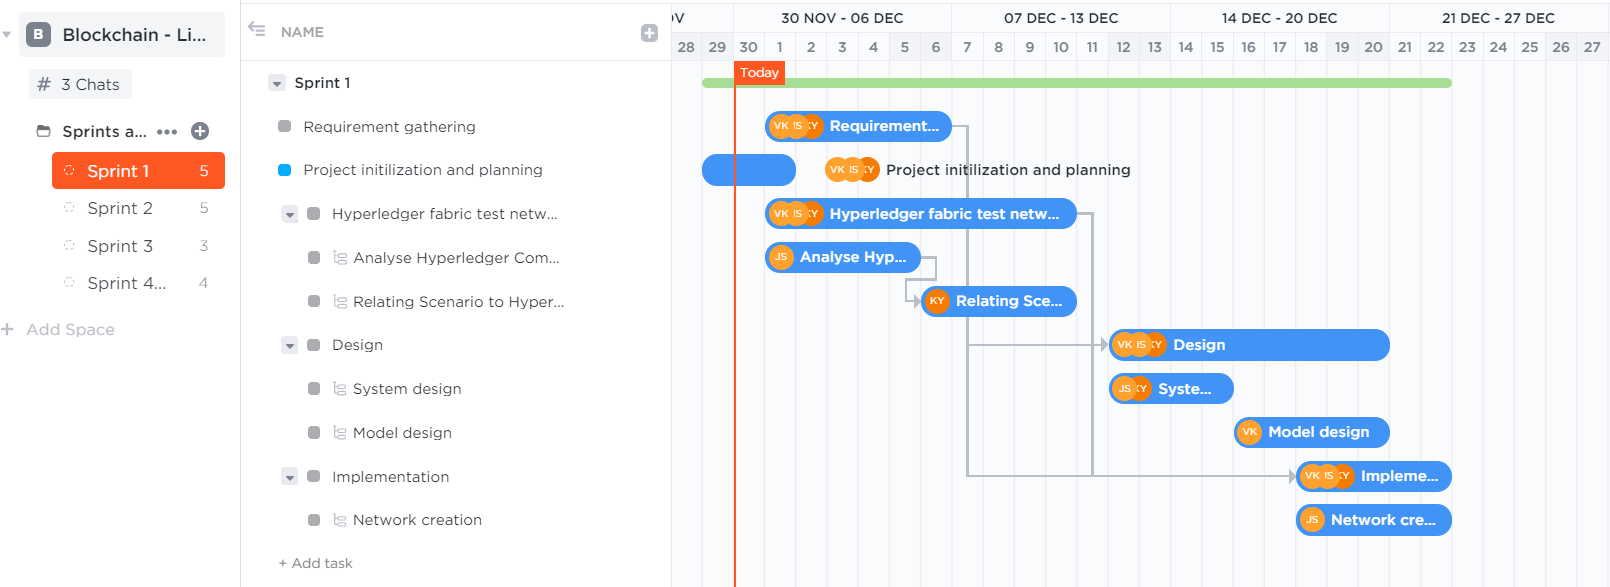
\includegraphics[height=6cm, width=11.5cm]{BC_Project_Plan.png}
        \end{center}
        \vspace{-3mm}
%\tiny Source: \texttt{https://hyperledger-fabric.readthedocs.io/en/latest/txflow.html}
\end{frame}



\section{References}

\begin{frame}
\frametitle{References}
\begin{thebibliography}{00}
\bibitem{b1} https://www.ncbi.nlm.nih.gov/pmc/articles/PMC7010942/
\bibitem{b2} https://www.ncbi.nlm.nih.gov/pmc/articles/PMC7474412/
\bibitem{b3} https://www.sciencedirect.com/science/article/pii/S2214212619306155
\bibitem{b4} https://hyperledger-fabric.readthedocs.io/ Accessed-On:01/12/2020
\bibitem{b5} https://medium.com/@lichunshen84/build-a-blockchain-poc-application-using-hyperledger-fabric-5a32687072b7, Accessed-On:01/12/2020
\end{thebibliography}

\end{frame}




\end{document}